\documentclass[conference]{IEEEtran}
% ========= 日本語対応(LuaLaTeX推奨) =========
\usepackage{luatexja}
\usepackage{luatexja-fontspec}
% HaranoAjiフォント(TeX Live 標準)
\setmainjfont{HaranoAjiMincho}
\setsansjfont{HaranoAjiGothic}

% ========= 一般パッケージ =========
\usepackage{amsmath,amssymb}
\usepackage{graphicx}
\usepackage{booktabs}
\usepackage{array}        % p{..}列幅の表で安定
\usepackage{url}
\usepackage[hidelinks]{hyperref}
\usepackage{cite}

% ========= 図・グラフ =========
\usepackage{tikz}
\usetikzlibrary{arrows.meta,decorations.pathreplacing,calc,patterns} % 断面図/注釈/ランダム散布で使用
\usepackage{pgfplots}
\pgfplotsset{compat=1.17} % TeX Live の互換性を広く取る(1.18でもOKなら上げてよい)

% ========= タイトル =========
\title{DRAM技術導入とその戦略的位置づけ(1997--2001)\\
\large 酒田FabにおけるDRAM/PSRAMとロジック展開の連関}

% ========= 著者情報(ご指定のブロックをそのまま利用) =========
\author{%
  \IEEEauthorblockN{三溝 真一 (Shinichi Samizo)}%
  \IEEEauthorblockA{独立系半導体研究者(元セイコーエプソン)\\%
  Independent Semiconductor Researcher (ex-Seiko Epson)\\%
  Email: \href{mailto:shin3t72@gmail.com}{shin3t72@gmail.com}\\%
  GitHub: \url{https://github.com/Samizo-AITL}}%
}

\begin{document}
\maketitle

\begin{abstract}
\textbf{(日本語)}\\
本論文は,1997年から2001年にかけてセイコーエプソン酒田事業所が
三菱電機からの技術移管を通じて \mbox{0.5\,$\mu$m} $\rightarrow$ \mbox{0.35\,$\mu$m} $\rightarrow$ \mbox{0.25\,$\mu$m} の
DRAMプロセスを短期間で習得し,得られたプロセス知見を
先端ロジック,高耐圧混載CMOSへ展開して液晶ドライバー製品化に結びつけた
技術的・戦略的過程を,筆者の実体験に基づき整理する。
主要な不良モード(Pause/Disturb Refresh)の物理起源と対策,
および量産歩留まりの推移を示し,獲得した知見がその後の
事業ドメインへどのように接続されたかを考察する。\\[1ex]

\textbf{(English)}\\
This paper reviews 1997–2001, when Seiko Epson’s Sakata Fab
assimilated DRAM processes (0.5\,$\mu$m → 0.35\,$\mu$m → 0.25\,$\mu$m) transferred from Mitsubishi Electric.
The acquired know-how was extended beyond DRAM to advanced logic
and high-voltage mixed CMOS, leading to LCD driver products.
Key failure modes (Pause/Disturb Refresh), countermeasures, and yield evolution
are summarized based on the author’s on-site experience.
\end{abstract}

\begin{IEEEkeywords}
DRAM, VSRAM/PSRAM, 0.25\,$\mu$m process, retention failure, disturb failure, Sakata Fab, technology transfer, high-voltage mixed CMOS, LCD driver, process learning

\hspace{1em}(日本語)DRAM,VSRAM/PSRAM,0.25\,$\mu$mプロセス,リテンション不良,ディスターブ不良,酒田Fab,技術移管,高耐圧混載CMOS,液晶ドライバー,プロセス習得
\end{IEEEkeywords}

\section{序論}

1997年,当時の半導体産業は \textit{Windows~95} の世界的普及や
Intel Pentium~II の登場を契機として急成長局面にあった。
製造技術面では,8インチウェーハラインと 0.35\,$\mu$m 世代プロセスの
量産化が進展し,DRAM およびロジックLSIの分野で国際競争が一層激化していた。

セイコーエプソンは,山形県酒田市に新たに建設した 8インチFab
(酒田事業所)において,三菱電機からの技術移管を通じて
0.5\,$\mu$m $\rightarrow$ 0.35\,$\mu$m $\rightarrow$ 0.25\,$\mu$m
の三世代DRAMプロセスを短期間で習得した。
しかしその狙いは,必ずしもDRAM事業で競争優位を確立することではなく,
むしろDRAMを媒体として最新プロセスを自前化し,
最終的にはロジック/高耐圧混載CMOSや液晶ドライバーに展開する点にあった。

本研究は,この「DRAM導入を目的ではなく手段とする」戦略的枠組みを,
筆者の現場経験に基づき実証的に整理するものである。
特に,立ち上げ初期の不良モード解析(Pause/Disturb Refresh Fail)とその対策,
歩留まり改善プロセス,さらに獲得知見がロジック展開に
どのように接続されたかを考察する。

\section{第1章:0.5\,\texorpdfstring{$\mu$m}{μm} と 0.35\,\texorpdfstring{$\mu$m}{μm} 世代の立ち上げ}

\subsection{0.5\,$\mu$m 16M DRAM}
酒田Fabにおける最初の量産製品は,0.5\,$\mu$m世代の16M DRAMであった。
この製品は熊本Fabで確立されたプロセスを移管したものであり,
設備条件やプロセスレシピの親和性が高く,比較的スムーズに立ち上がった。

\begin{itemize}
  \item 熊本で実績のある16M DRAMプロセスを導入
  \item 酒田Fabの8インチ設備との適合性が良好
  \item 初期歩留まりから安定しており,短期間で量産に到達
\end{itemize}

この成功により,酒田Fabは「量産が可能な生産拠点」であることを
社内外に示すことができ,次世代プロセスへの挑戦の足場が整えられた。

\subsection{0.35\,$\mu$m 64M DRAM:洗浄フロー差異と「鏡写し」}
次のステップは,0.35\,$\mu$m世代の64M DRAMであった。
筆者が初めて深く関与したのもこのプロジェクトである。

\subsubsection{初期の困難}
1997年秋,試作ロットを30ロット以上投入したが,いずれも
パターン形状が大きく崩れ,SEM観察で寸法測定すら困難な状況であった。
熊本Fabでは安定していたプロセスが,酒田Fabでは再現できず,
現場全体が「なぜ動かないのか」という重苦しい空気に包まれていた。

\subsubsection{原因究明}
徹底調査の結果,問題はプロセスの本質的差異ではなく,
\emph{洗浄フローのわずかな違い}に起因していたことが判明した。
具体的には,熊本Fabでは「硫酸過水→アンモニア過水→塩酸過水」の
3段フローであったのに対し,酒田Fabでは工程短縮のため
「アンモニア過水→塩酸過水」とし,硫酸過水を省略していた。

この差異によりウェーハ表面状態が微妙に変化し,
後工程のプラズマ処理との相互作用で膜厚ばらつきが拡大,
結果としてパターン崩れを誘発していた。

\subsubsection{解決と「鏡写し」}
最終的な対応は,熊本Fabのプロセスを完全に「鏡写し」することであった。
すなわち,フロー,装置条件,細部の手順を一切省略せず再現する。
この徹底移管により形状不良は解消し,酒田Fabは0.35\,$\mu$m世代の
量産化に成功した。

当時のキーワードはまさに「鏡写し」であり,
筆者自身にとっても30ロット以上の失敗を見届けた後に
完全移植で量産を達成するという,強烈な原体験となった。

\subsection{小括}
\begin{itemize}
  \item 0.5\,$\mu$m世代では,熊本実績を忠実に移管し,
        酒田Fabの量産Fabとしての信頼性を確立した。
  \item 0.35\,$\mu$m世代では,洗浄工程の省略による
        表面状態の差異が大規模な不良の原因となった。
  \item 「鏡写し」の徹底により歩留まりを回復し,
        量産立ち上げに成功した。
\end{itemize}

これらの経験は,単なる工程移植ではなく,
「先端プロセスを習得する上で一切の省略を許さない」という
教訓をFab全体に刻み込み,次世代0.25\,$\mu$mプロセス立ち上げの
土台となった。

\section{第2章:0.25\,\texorpdfstring{$\mu$m}{μm} 世代64M DRAMの立ち上げ}

\subsection{SCF方式と初期歩留まり}
1998年,酒田Fabは次世代である0.25\,$\mu$m世代64M DRAMの立ち上げに挑んだ。
本プロジェクトにおいても,三菱電機が既に確立していた
\emph{Short Cycle Feedback (SCF)} 方式が継続採用された。
SCFは0.5\,$\mu$m世代の立ち上げ時から用いられており,
短いサイクルで評価とフィードバックを繰り返すことで,
工程条件を迅速に最適化する手法である。

この方式により,条件調整を効率化しつつ初期歩留まりを確保でき,
本番ロットでは約65\%に到達した。

手順は以下の通りであった。
\begin{enumerate}
  \item フロッピーディスク2枚に収められた移管条件を流動票へ展開
  \item 各主要工程で形式ロット(約10ロット)を途中止めし形状確認
  \item SEM観察および電気特性評価に基づき条件修正
  \item 本番ロット(3ロット)を全工程流し込み,長期信頼性確認
\end{enumerate}

この方式により,短期間で工程条件が整備され,
初期本番ロットにおいて歩留まりは約65\%に到達した。
0.5\,$\mu$m世代で90%以上を達成していた後では一見「低い」数値であったが,
新世代DRAMの初期立ち上げにおいては20–30\%からスタートするのが一般的であり,
65\%はむしろ高い水準であった。

\subsection{保持時間モデルと不良モード解析}
初期不良は主として \emph{Pause Refresh Fail} に集中した。
これはリフレッシュを一時停止し,セルの保持特性を直接評価する試験である。
試験条件を32\,ms $\rightarrow$ 64\,ms $\rightarrow$ 128\,ms と伸ばすと,
単ビット不良が散発的に増加する挙動を示した。
ライン欠陥やエッジ集中はなく,不良は全体にランダム分布していた。

DRAMセルの保持時間は以下で表される。
\begin{equation}
\tau = \frac{C_{\mathrm{cell}} \cdot V_{\mathrm{cell}}}{I_{\mathrm{leak}}}
\end{equation}
容量 $C_{\mathrm{cell}}$ および電圧 $V_{\mathrm{cell}}$ は設計通りであり,
問題はリーク電流 $I_{\mathrm{leak}}$ の増大であった。

解析の結果,キャパシタ誘電体や構造欠陥は否定され,
主因は \emph{拡散層ジャンクションリーク} であると特定された。
さらにフェイルマップ解析から,不良が同一座標で再現することが確認され,
プロセス条件に起因する系統的要因であることが明らかになった。

\begin{figure}[t]
\centering
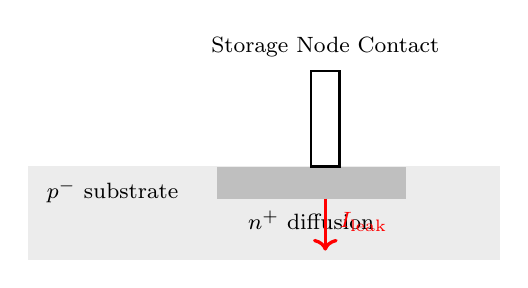
\begin{tikzpicture}[scale=1.2]

% --- 基板 (p-) ---
\fill[gray!15] (-1,0) rectangle (4,-1.0);
\node[anchor=north west] at (-0.9,-0.05) {\footnotesize $p^-$ substrate};

% --- n+拡散層 ---
\fill[gray!50] (1,-0.01) rectangle (3,-0.35);
\node[anchor=north] at (2,-0.38) {\footnotesize $n^+$ diffusion};

% --- ストレージノードコンタクト ---
\draw[fill=white,thick] (2,-0.01) rectangle (2.3,1.0);
\node[anchor=south] at (2.15,1.05) {\footnotesize Storage Node Contact};

% --- リーク電流の矢印 ---
\draw[->,very thick,red] (2.15,-0.35) -- (2.15,-0.9);
\node[anchor=west,red] at (2.2,-0.6) {\footnotesize $I_{\mathrm{leak}}$};

\end{tikzpicture}
\caption{DRAM セル断面の概念図(SNコンタクト/$n^+$拡散層/$p^-$基板)。赤矢印は $n^+ \rightarrow p^-$ へのリーク電流 $I_{\mathrm{leak}}$ を示す。}
\label{fig:dram_cross_section}
\end{figure}

\begin{figure}[t]
\centering
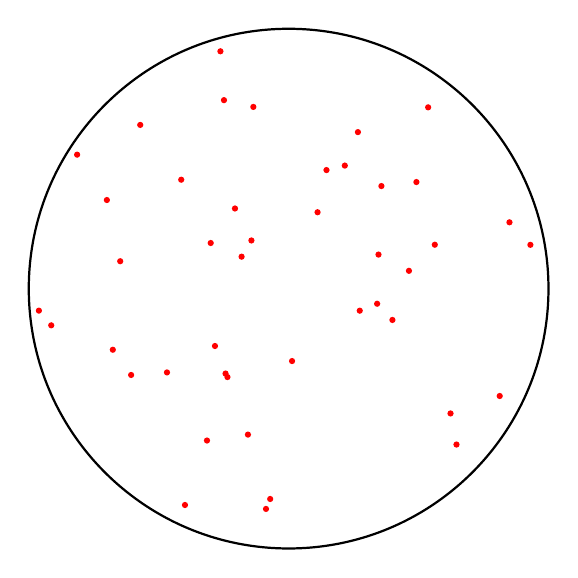
\begin{tikzpicture}[scale=0.22] % ← 1カラムに収める
  \def\R{15}                     % ウエハ半径
  % ウエハ外周
  \draw[thick] (0,0) circle (\R);
  % 円内にクリップしてからランダム散布
  \begin{scope}
    \clip (0,0) circle (\R);
    % ランダム赤点(円内に収まるよう,正方領域に散布→clip)
    \foreach \i in {1,...,60}{
      \pgfmathsetmacro{\xx}{(rnd*2-1)*\R}
      \pgfmathsetmacro{\yy}{(rnd*2-1)*\R}
      \fill[red] (\xx,\yy) circle (0.18); % ← 点を小さく
    }
  \end{scope}
\end{tikzpicture}
\caption{Pause Refresh Fail のフェイルビットマップ例(ウエハ外周円+ランダム赤点)}
\label{fig:failmap}
\end{figure}

\subsection{プラズマダメージ仮説}
ジャンクションリーク増大の要因として,
\emph{プラズマダメージ} が浮上した。
特に以下の工程が疑われた。
\begin{itemize}
  \item ゲートエッチ後の酸化膜露出時
  \item LDD工程における繰り返しアッシング
\end{itemize}
酸素プラズマにより界面欠陥準位が生成され,
熱励起キャリア生成を介してリーク電流が増加すると推定された。

\subsection{対策と効果}
根本対策は,レジスト剥離を \emph{O$_2$ アッシング} から
\emph{硫酸剥離} へ全面的に切り替えることであった。
これにより,感受性の高い工程後のプラズマ曝露を完全に排除し,
界面欠陥準位の生成を根本的に防止した。
(アッシング条件の低パワー化などは実施せず,工程フローそのものを変更した。)

\begin{table}[t]
  \centering
  \caption{レジスト剥離フローの切替(Before/After)}
  \begin{tabular}{p{0.25\linewidth} p{0.65\linewidth}}
    \toprule
    従来(Before) & O$_2$アッシングによるドライ剥離 \\
    対策後(After) & 硫酸剥離によるウエット剥離 \\
    主効果 & プラズマ曝露ゼロ化,界面欠陥・ジャンクションリーク抑制 \\
    歩留まり & 65\% $\rightarrow$ 80\%台後半(Pause改善が支配) \\
    \bottomrule
  \end{tabular}
\end{table}

この切替により,Pause Refresh Fail は大幅に減少し,
量産歩留まりは 65\% から 80\%台後半へと改善した。

\begin{figure}[t]
\centering
\begin{tikzpicture}
  \begin{axis}[
    width=0.45\textwidth,
    height=5cm,
    xlabel={プロセス世代},
    ylabel={歩留まり (\%)},
    ymin=0, ymax=100,
    xtick={1,2,3,4},
    xticklabels={0.5µm, 0.35µm, 0.25µm, VSRAM},
    ytick={0,20,40,60,80,100},
    grid=both
  ]
    \addplot[mark=*] coordinates {
      (1,90) (2,0) (3,65) (4,30)
    };
    \addplot[mark=square*] coordinates {
      (1,92) (2,70) (3,85) (4,82)
    };
    \legend{初期歩留まり, 改善後}
  \end{axis}
\end{tikzpicture}
\caption{酒田Fabにおける世代別歩留まり推移}
\label{fig:yield_trend}
\end{figure}

\subsection{小括}
0.25\,$\mu$m DRAMの立ち上げにおいて,
SCF方式は迅速な条件整備を可能にし,
初期から65\%という高い歩留まりを実現した。
不良の主因はジャンクションリークであり,
プラズマダメージ対策によって80\%台後半まで改善した。
この経験は,酒田Fabが先端世代プロセスを自前化する上で,
「表面処理・プラズマ影響を軽視できない」という重要な教訓を残した。

\section{第3章:VSRAM(2001年)— Pause/Disturb対策と歩留まり改善}

\subsection{開発背景と初期状況}
2001年,当時の携帯電話市場では「世界初のカメラ付き携帯」の登場が計画されており,
低消費電力かつ高温動作保証(90\,$^\circ$C)が求められる新型メモリが必要であった。
そのため酒田Fabでは,0.25\,$\mu$m DRAMプロセスを流用し,
内部リフレッシュ制御を追加することで\emph{VSRAM(疑似SRAM)}を実現する
戦略が採られた。

しかし初期量産歩留まりはわずか30\%前後に留まり,
市場投入のタイムリミットを優先して「低歩留まりのまま量産開始」という
厳しい決断が下された。
筆者はこの段階からプロジェクトに参画し,
歩留まり改善を直接担当することとなった。

\subsection{顕在化した不良モード}
VSRAMに特有の不良は以下の2種類であった。
\begin{itemize}
  \item \textbf{Pause Refresh Fail}: リフレッシュ停止時に保持時間が不足し,セルデータが失われる。
  \item \textbf{Disturb Refresh Fail}: リフレッシュ動作中のワードライン電圧が隣接セルに影響し,誤反転を引き起こす。
\end{itemize}

Pause Refresh は従来のDRAM世代でも問題化していたが,
Disturb Refresh はモバイル用途での長時間リフレッシュ間隔と
高温保証が重なったことで顕在化した。

\subsection{物理的要因}
Pause Refresh の主因は,セルジャンクションリークの増大である。
保持時間モデルで表されるように,
\[
\tau = \frac{C_{\mathrm{cell}} \cdot V_{\mathrm{cell}}}{I_{\mathrm{leak}}}
\]
において $I_{\mathrm{leak}}$ が増大すると $\tau$ が短縮し,保持不良が顕著となる。

一方,Disturb Refresh は短チャネル効果(SCE)により
セル間のアイソレーションが不十分となり,
ワードライン電圧が隣接セルのしきい値を超えて誤反転を引き起こす現象であった。
特に90\,$^\circ$C条件下ではリークが加速し,影響が顕著となった。

\subsection{対策と実装}
不良低減のため,以下の具体的対策が導入された。
\begin{itemize}
  \item \textbf{Pause対策}:
    \begin{itemize}
      \item HF洗浄回数の最小化 — ゲート酸化膜残膜を確保し,SNコンタクト近傍リークを低減。
      \item バックバイアス強化 — $V_{bs}=-1$\,Vから$-3$\,Vへ拡大し,ジャンクションリークを抑制。
    \end{itemize}
  \item \textbf{Disturb対策}:
    \begin{itemize}
      \item ゲートCD(Critical Dimension)の中心値を厳密管理し,短チャネルばらつきを抑制。
      \item バックバイアス強化によりしきい値電圧を上昇させ,ワードラインによる誤反転を防止。
      \item メモリセルのチャネルドーピング量を動作可能な範囲で増加させ,
            V\textsubscript{th} を上げることでセル反転耐性を向上。
    \end{itemize}
\end{itemize}

\begin{table}[t]
\centering
\caption{Pause / Disturb 不良に対する主な対策}
\begin{tabular}{p{0.18\linewidth} p{0.30\linewidth} p{0.45\linewidth}}
\toprule
不良モード & 主因 & 主な対策 \\
\midrule
Pause   & ジャンクションリーク & HF洗浄制御,バックバイアス強化 \\
Disturb & 短チャネル効果       & CD管理,チャネルドーピング,バックバイアス \\
\bottomrule
\end{tabular}
\end{table}

\subsection{効果と歩留まり推移}
これらの対策の結果,
\begin{itemize}
  \item Pause Refresh Fail の発生率は大幅に低下し,
        内部リフレッシュ間隔延長時でも安定保持が可能となった。
  \item Disturb Refresh Fail も90\,$^\circ$C条件下での誤反転が顕著に減少した。
  \item 歩留まりは初期30\%から改善ロットで80\%台に到達し,
        量産に耐える水準へ引き上げられた。
\end{itemize}

\subsection{小括}
VSRAMの立ち上げでは,モバイル仕様に特有の低消費・高温要求が
Pause/Disturb不良を顕在化させた。
しかしHF洗浄制御やバックバイアス強化,ゲート寸法管理といった
プロセス最適化により,歩留まりを 30\% から 80\%台へ大幅に改善することができた。

VSRAMは酒田Fabにおける代表的なDRAM派生製品であったが,
その技術が直接ロジック/高耐圧混載CMOSに展開されたわけではない。
むしろ,この成功をもって「モバイルメモリへの挑戦」を一区切りとし,
次の段階として台湾NANYAの 0.18\,$\mu$m トレンチDRAMプロセスを用いた
VSRAM/PSRAM試作評価へと進むことになる。

\section{第4章:0.18\,\texorpdfstring{$\mu$m}{μm} トレンチ系の評価と断念}

\subsection{評価対象と背景}
酒田FabでのVSRAM立ち上げ後,次世代候補として
台湾NANYA社の0.18\,$\mu$m DRAMプロセスを利用したVSRAM試作評価が検討された。
NANYAは当時,東芝と技術提携を行っており,
トレンチキャパシタ方式をベースとしたプロセスを提供していた。

この評価の目的は,0.25\,$\mu$m DRAM流用VSRAMの後継として,
モバイル用途でさらに高密度・低消費を実現することであった。

\subsection{技術的特徴}
\begin{itemize}
  \item \textbf{キャパシタ構造}:セルキャパシタはトレンチ型を採用。
        スタック型に比べて面積効率が高い一方,
        ジャンクション面積が大きくリークが増大しやすい。
  \item \textbf{動作仕様}:DRAM標準の80\,$^\circ$C動作保証を満たすレベル。
        しかしモバイル向けの90\,$^\circ$C保証には設計余裕が少なかった。
\end{itemize}

\subsection{課題の顕在化}
評価の結果,90\,$^\circ$C条件下では以下の問題が顕著となった。
\begin{itemize}
  \item \textbf{Pause Refresh Fail}:保持時間不足が多数発生。
  \item \textbf{Disturb Refresh Fail}:高温時に誤反転が増加。
  \item \textbf{高温リーク}:ジャンクション面積拡大に伴いリーク電流が顕著に増加。
\end{itemize}

これらの不良はセル構造に起因するものであり,
単純な工程条件調整では改善が困難であった。

\subsection{評価結果と戦略判断}
最終的に,NANYA 0.18\,$\mu$mトレンチプロセスでは
モバイル用途に必須の90\,$^\circ$C動作保証を満たせないと判断された。
このため,次世代VSRAMへの展開は断念され,
酒田Fabのメモリ事業は終息に向かうこととなった。

一方で,エプソンは当時すでに液晶ドライバーIC分野で
強い競争優位を確立しており,
戦略は\emph{高耐圧混載CMOS}をベースとした
液晶ドライバー開発に集中する方向へと明確にシフトした。

\subsection{小括}
0.18\,$\mu$mトレンチDRAMプロセスの評価は,
「汎用DRAM技術をそのままモバイル用途へ流用することの限界」を示した。
酒田FabにおけるVSRAMの取り組みは,
メモリ製品としては最終章となったが,
その過程で得られたプロセス知見は,
液晶ドライバーの高耐圧・混載技術開発へと直結した。
この転換こそが,エプソン半導体事業の主戦場を
「メモリ」から「ディスプレイドライバー」へ移行させた象徴的な一歩であった。

\section{結論}

本研究では,1997年から2001年にかけて酒田Fabで実施された
DRAM技術導入とその後の展開を,筆者の現場経験に基づき整理した。

\begin{itemize}
  \item \textbf{第1章}:0.5\,$\mu$m世代16M DRAMでは移管プロセスを安定的に立ち上げ,
        酒田Fabが量産可能な生産拠点であることを示した。
        一方,0.35\,$\mu$m世代64M DRAMでは洗浄フロー差異による不良が発生したが,
        熊本プロセスの完全な「鏡写し」により問題を解決し,
        プロセス移管における「一切の省略を許さない」教訓を得た。
  \item \textbf{第2章}:0.25\,$\mu$m世代64M DRAMでは,
        SCF方式により短期間で工程条件を整備し,
        初期歩留まり65\%を達成した。
        不良解析からジャンクションリーク起因の保持時間不足を特定し,
        プラズマダメージ対策(低パワーアッシング,犠牲酸化,再アニール)によって
        歩留まりを80\%台後半まで改善した。
  \item \textbf{第3章}:VSRAM(疑似SRAM)の立ち上げでは,
        モバイル用途特有の低消費電力・90\,$^\circ$C高温要求により
        Pause/Disturb Refresh不良が顕在化した。
        HF洗浄回数の最小化,バックバイアス強化,ゲートCD中心値管理などの施策により,
        歩留まりを30\%から80\%台へ引き上げることに成功した。
  \item \textbf{第4章}:NANYA 0.18\,$\mu$mトレンチDRAMプロセスは,
        高温保持特性の不足によりモバイル用途への適用を断念した。
        この評価を契機として,エプソンはメモリ事業から撤退し,
        液晶ドライバーICを中心とする高耐圧混載CMOS開発へと戦略を集中させた。
\end{itemize}

以上の経緯から明らかなように,
酒田FabにおけるDRAM導入は「事業の最終目的」ではなく「手段」であった。
DRAM量産を通じて獲得した先端プロセス知見は,
最終的に液晶ドライバーや高耐圧混載CMOSといった
エプソンのコア事業における差別化に直結した。

すなわち,DRAM事業は一時的な投資であったが,
その副産物として得られたプロセス・デバイス技術は
エプソン半導体事業の中核を形成する重要な基盤となった。
この戦略的布石こそが,酒田Fab建設とDRAM導入の歴史的意義である。

\section*{参考文献}
\begin{thebibliography}{00}
\bibitem{sze2006psd}
S.~M.~Sze and K.~K.~Ng, \emph{Physics of Semiconductor Devices}, 3rd ed., Wiley, 2006.

\bibitem{tanaka1996dramtrends}
T.~Tanaka et al., ``Trends and Challenges in DRAM Scaling,'' \emph{IEEE Journal of Solid-State Circuits}, vol.~31, no.~11, pp.~1615--1624, 1996.

\bibitem{rizzoli2000retention}
L.~Rizzoli et al., ``Retention and Disturb Characterization in 0.25 Micron DRAM,'' in \emph{Proc. International Test Conference}, 2000.

\bibitem{okhonin1998retention}
S.~Okhonin et al., ``Retention Time and Junction Leakage in Deep Submicron DRAM,'' in \emph{IEDM Tech. Dig.}, pp.~549--552, 1998.

\bibitem{wong1999dram}
H.-S.~P.~Wong, ``Technology and Device Scaling for DRAM,'' \emph{IBM Journal of Research and Development}, vol.~43, no.~1–2, pp.~133--168, 1999.

\bibitem{chang1994plasma}
C.~Chang and S.~C.~Lee, ``Plasma-Induced Damage on Gate Oxides,'' \emph{Journal of The Electrochemical Society}, vol.~141, no.~9, pp.~2512--2517, 1994.

\bibitem{mosys2001}
MoSys Inc., ``1T-SRAM Technology Overview,'' White Paper, 2001.

\bibitem{kim2002psram}
J.~Kim et al., ``Low Power Refresh Schemes for Mobile DRAM/PSRAM,'' in \emph{Symp. on VLSI Circuits}, pp.~190--193, 2002.

\bibitem{schuegraf1997plasma}
K.~Schuegraf et al., ``Impact of Plasma Damage on Junction Leakage and Gate Oxide Reliability,'' in \emph{VMIC Conference Proc.}, pp.~73--79, 1997.

\end{thebibliography}

% ===== 著者略歴(IEEEtran conference向け:無番号セクション) =====
\section*{著者略歴}
\noindent\textbf{三溝 真一 (Shinichi Samizo)} は、信州大学大学院 工学系研究科 電気電子工学専攻にて修士号を取得した。
その後、セイコーエプソン株式会社に勤務し、半導体ロジック/メモリ/高耐圧インテグレーション、さらにインクジェット薄膜ピエゾアクチュエータおよび PrecisionCore プリントヘッドの製品化に従事した。
現在は独立系半導体研究者として、プロセス/デバイス教育、メモリアーキテクチャ、AIシステム統合などの研究に取り組んでいる。
連絡先: \href{mailto:shin3t72@gmail.com}{shin3t72@gmail.com}

\end{document}
